\section{Class-dependent sigmoid loss for PU Learning}
\label{sec:pulearning}


%%%%%%%%%%%%%%%%%%%%%%%%%%%%%%%%%%%%%%%%%%%%%%%%%%%%%%%%%%%%%%%%%%%%%%
%%%%%%%% FIGURE Losses
%%%%%%%%%%%%%%%%%%%%%%%%%%%%%%%%%%%%%%%%%%%%%%%%%%%%%%%%%%%%%%%%%%%%%%

\begin{figure}[t]
\centering
\textbf{Losses and derivatives}\par\medskip
% \fbox{\rule{0pt}{2in} \rule{0.9\linewidth}{0pt}}
   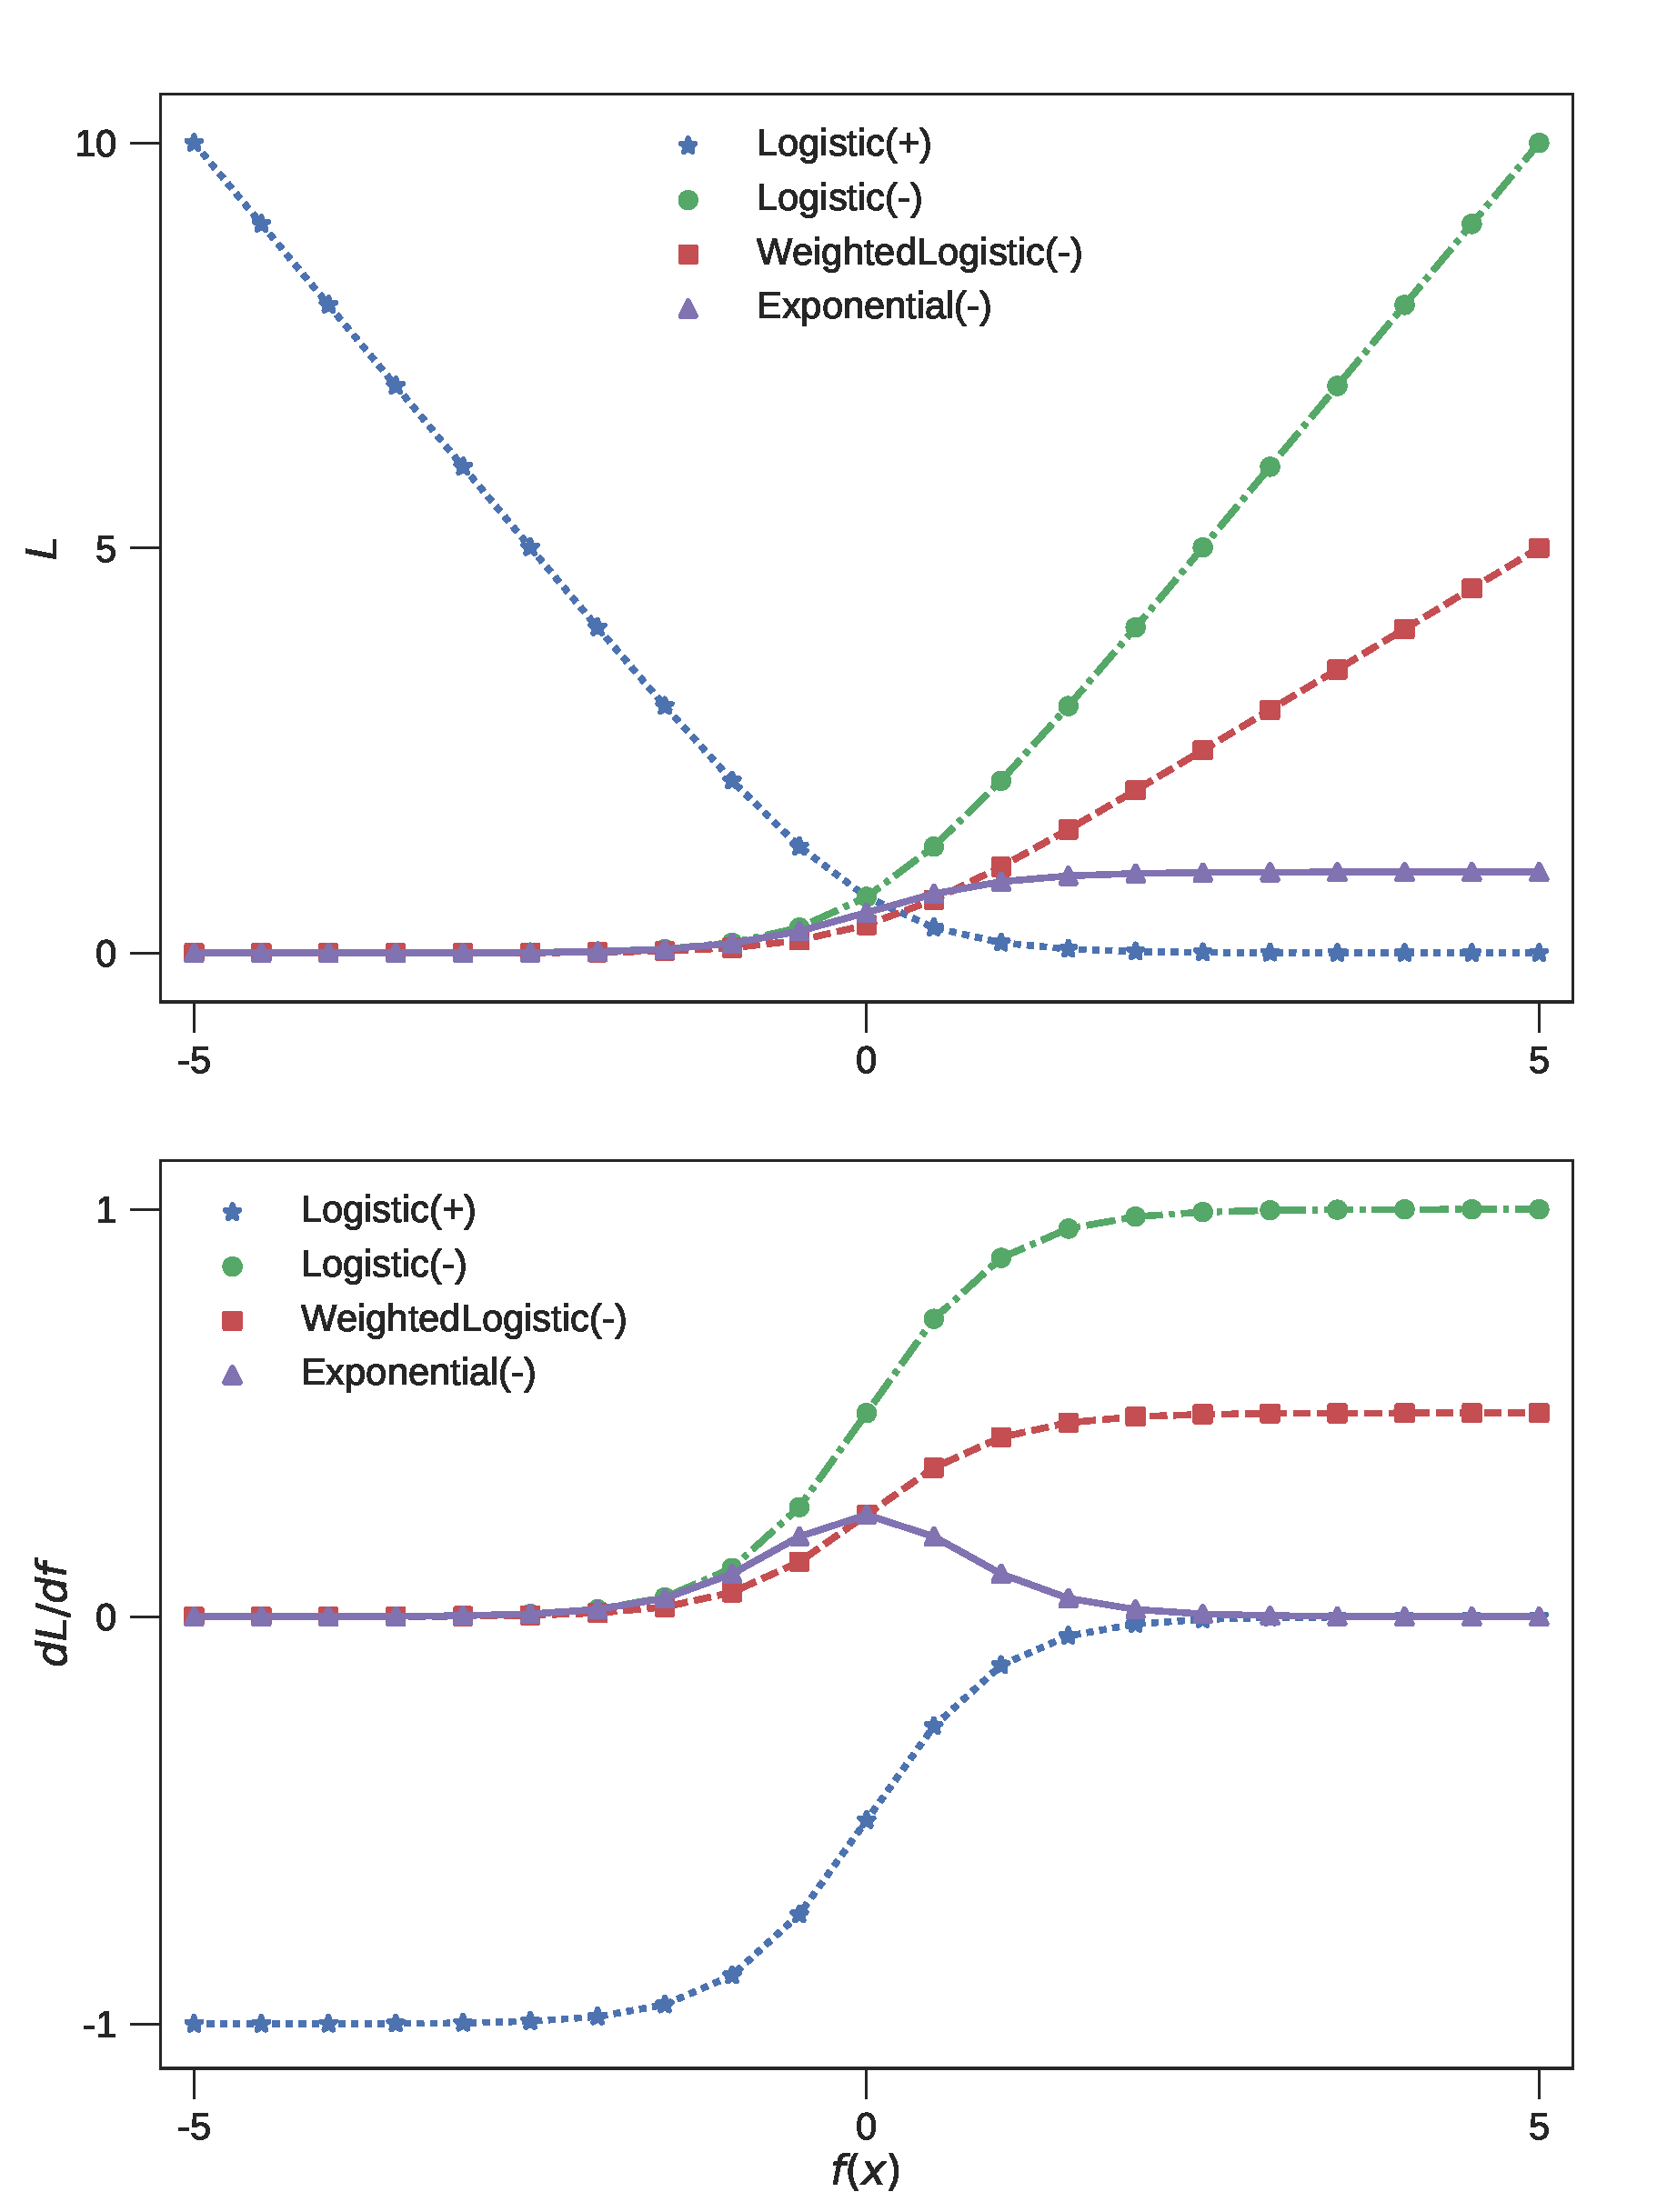
\includegraphics[width=1.05\linewidth]{img/losses}
\caption{
The differences in losses (left figure) and derivatives (right figure) with respect to the model $f$ between the weighted logistic loss and the sigmoid loss for the negative class.
The $x$-axis denotes the model output $f(x)$, varying from negative infinity to positive infinity.
We present only $(-5,5)$ for compact figures.
The \textbf{+} sign represents the loss of positive samples, and the \textbf{-} sign stands for the loss of negative samples.
The sigmoid loss of negative examples reaches a plateau and the derivative drops to zero in the region of large $f(x)$, whereas the weighted logistic loss for negative is a linearly scaled logistic loss.
The sigmoid loss fulfills the requirement of not punishing the model more for more positive output than less positive output.
}
\label{fig:losses}
\end{figure}


%%%%%%%%%%%%%%%%%%%%%%%%%%%%%%%%%%%%%%%%%%%%%%%%%%%%%%%%%%%%%%%%%%%%%%
%%%%%%%% TEXT Weighted loss for negatives
%%%%%%%%%%%%%%%%%%%%%%%%%%%%%%%%%%%%%%%%%%%%%%%%%%%%%%%%%%%%%%%%%%%%%%

In this section, we introduce losses for learning with positive and unlabeled examples.

\paragraph{Class-weighted loss}

A class-weighted logistic loss $l_{weighted}(\cdot)$ for a pair of input feature and observed label $(x, y)$ with a model $f(\cdot)$ parametrized by $\theta$ is:
\begin{eqnarray}
\resizebox{0.9\columnwidth}{!}{$
l_{weigted}(x, y; \theta) =
  \begin{cases}
    - \alpha \log (\sigma(f(x; \theta))) , & y = +1 \\
    - \beta \log (1 - \sigma(f(x; \theta))), & y = -1,
    % - \alpha \log P(y=+1 \vert x; \theta), & y = +1 \\
    % - \beta \log P(y=-1 \vert x; \theta), & y = -1
  \end{cases}
$}
\end{eqnarray}
where $\alpha$ and $\beta$ are weights for positive and negative class respectively, and $\sigma(\cdot)$ is the sigmoid function.
This loss is referred to as the \textbf{class-weighted loss} in the rest of paper.
Empirically, the choice of $\alpha$, $\beta$ can be made based on the highest precision and recall achieved on a validation set, or based on a class priors estimation\cite{du2014class}.
% Alternatively, one can also roughly assign $q=p(y=-1 \vert \tilde{y}=-1)$.
% This turns out to be part of the backward corrected loss proposed in  \cite{patrini2016making}:
% \begin{equation*}
%   \begin{aligned}
%     l_{\tilde{y_i}=-1} = - p(y_i=-1 \vert \tilde{y_i}=-1) \log p(y_i=-1 \vert x_i) \\ - p(y_i=+1 \vert \tilde{y_i}=-1) \log p(y_i=+1 \vert x_i)
%   \end{aligned}
% \end{equation*}
% % $$p( \tilde{y} \vert x, y) = \sum_{y}p(\tilde{y} \vert y)p(y \vert x)$$
% % $$p(y=+1 \vert \tilde{y}=+1) = 1 $$
% % $$p(y=-1 \vert \tilde{y}=+1) = 0 $$
% with $p(y_i=-1 \vert \tilde{y_i}=-1) = q$ and $p(y_i=+1 \vert \tilde{y_i}=-1) = 1-q$.


We extend the class-weighted logistic loss to a class-weighted cross entropy for multiclass classification with $K$ relevant classes and one one-relevant class (class $0$).
Suppose there are K relevant categories and one non-relevant categories, the corresponding class-weighted loss $l_{wtd}$ for a training sample $(x,y)$ with a model $f(\cdot)$ parametrized by $\theta$ is:
\begin{eqnarray}
\resizebox{0.9\columnwidth}{!}{$
l_{weighted}(x, y; \theta) =
  \begin{cases}
    - \beta  \log (\sigma_0(f(x;\theta))), & y = 0 \\
    - \alpha_1 \log (\sigma_1(f(x;\theta))), & y = 1 \\
                                            & \vdots \\
    - \alpha_K \log (\sigma_K(f(x;\theta))), & y = K,
  \end{cases}
$}
\end{eqnarray}
where $\alpha_1, \dots, \alpha_K, \beta$ are the weighting factors, $\sigma_0, \dots, \sigma_K$ are the softmax functions for class $0$ to $K$ respectively.
This loss is referred to as the \textbf{class-weighted cross-entropy}.


%%%%%%%% TEXT sigmoid Negative loss
\paragraph{Sigmoid/softmax Loss for the negative class}

The class-dependent sigmoid loss $l_{sigmoid}$ a sigmoid loss for the negative class and keep the loss for the positive class unchanged uses a logistic loss, for example, a logistic loss:
\begin{eqnarray}
\resizebox{0.9\columnwidth}{!}{$
l_{sigmoid}(x, y; \theta) =
  \begin{cases}
    - \log (\sigma(f(x; \theta))) , & y = +1 \\
    \sigma(f(x; \theta)), & y = -1,
    % - \log P(y=+1 \vert x; \theta), & y = +1 \\
    % 1 - P(y=-1 \vert x; \theta), & y = -1
  \end{cases}
$}
\end{eqnarray}
where $(x, y)$ is a pair of input feature and label, and $f(\cdot;\theta)$ is the model parametrized by $\theta$, and $\sigma(\cdot)$ is the sigmoid function.
This loss is referred as the \textbf{class-dependent sigmoid loss} or the \textbf{sigmoid loss} in short, in a sense it uses a sigmoid function for the negative class only.

Figure \ref{fig:losses} shows the sigmoid loss reaches a plaetau when the model output $f(x)$ grows above $2$, and its derivatives with respect to the model $f$ drops zero.
By contrast, the weighted logistic loss, with $\alpha=1$ and $\beta=0.5$, for the negative class is scaled by a factor of $0.5$ compared to the normal logistic loss for the negative class.
It keeps growing with a rate of $0.5$ as $f(x)$ grows in the large $f(x)$ area.
A large output $f(x)$ represents that the model is more confident for the corresponding example being positive.
The sigmoid loss follows our idea of not punishing highly confident positive predictions more than positive predictions with less confidence, whereas the weighted loss does not.

The class-dependent sigmoid loss is extendable to a multiclass scenario where $K$ is the number of relevant classes and $0$ denotes the non-relevant class.
The corresponding loss $l_{softmax}$ for an example, label pair $(x,y)$ with a model $f(\dot;\theta)$ is:
\begin{eqnarray}
\resizebox{0.9\columnwidth}{!}{$
l_{softmax}(x, y; \theta) =
  \begin{cases}
    1 - \sigma_0(f(x;\theta))), & y = 0 \\
    - \log (\sigma_1(f(x;\theta))), & y = 1 \\
                                   & \vdots \\
    - \log (\sigma_K(f(x;\theta))), & y = K,
  \end{cases}
  $}
\end{eqnarray}
where $\sigma_0, \dots, \sigma_K$ are the softmax functions for class $0$ to $K$ respectively.
This loss is called the \textbf{class-dependent softmax loss} or the \textbf{softmax loss} for simplicity.

%%%%%%%% TEXT Bootstrapping
\paragraph{Hard bootstrapping loss for the negative class}
In addition to the proposed sigmoid loss, we also modify the hard bootstrapping loss by Reed et al. \cite{reed2014training} for PU learning to set a benchmark.
The modified class-dependent hard bootstrapping loss for a pair of inputs and label $(x,y)$ with a model $f(\cdot;\theta)$ is:
\begin{eqnarray}
\resizebox{0.9\columnwidth}{!}{$
  l_{bootstrap}(x, y; \theta) =
    \begin{cases}
      - \log (\sigma_{+1}(f(x; \theta))) , & y = +1 \\
      - \beta \log (\sigma_{-1}(f(x; \theta))) - (1-\beta) \log (\sigma_{\hat{y}}(f(x; \theta))), & y = -1,
    \end{cases}
$}
\end{eqnarray}
where $\hat{y} = \argmax_{j\in\{-1,+1\}}{\sigma_{j}(f(x; \theta))}$ is the class with the highest predicted probability and $0<\beta<1$ is a hyperparameter to tune.
The first term of the loss for the negative class is a weighted logistic loss and the second term can be considered as a regularization term to encourage consistent predictions.
This loss is referred as the \textbf{bootstrapping loss} for the rest of this paper.
% \begin{equation*}
%   \begin{aligned}
%     H = - \sum_{j\in\{-1,+1\}} p(y_i=j \vert x_i) \log p(y_i=j \vert x_i) \\
%     \sim - \sum_{j\in\{-1,+1\}} \delta(y_i - \hat{y_i}) \log p(y_i=j \vert x_i)
%   \end{aligned}
% \end{equation*}
% which intuitively encourages the model to make confident predictions \cite{grandvalet2005semi}.

Similarly as the weighted loss and the sigmoid loss, this hard bootstrapping loss $l_{bootstrap}$ can be extended to multiclass:
\begin{eqnarray}
\resizebox{0.9\columnwidth}{!}{$
l_{bootstrap}(x, y; \theta) =
  \begin{cases}
    - \beta \log (\sigma_{0}(f(x; \theta))) - (1-\beta) \log (\sigma_{\hat{y}}(f(x; \theta))), & y = 0 \\
    - \log (\sigma_1(f(x;\theta))), & y = 1 \\
                                   & \vdots \\
    - \log (\sigma_K(f(x;\theta))), & y = K,
  \end{cases}
  $}
\end{eqnarray}
where $f(\cdot)$ is the model parametrized by $\theta$, and $\sigma_0, \dots, \sigma_K$ are the softmax functions for class $0$ to $K$ respectively, and $(x,y)$ is a pair of example and label, and $K$ is the number of relevant class while $0$ is the non-relevant class, and lastly $0<\beta<1$ is a hyperparameter.


%%%%%%%% TEXT Expontial loss FADE IN
\paragraph{Implementation details}
For all losses being used to learning with positive and unlabeled data, we reweighed the positive and negative class based on their occurrences in the observed labels to alleviate the influence of imbalance introduced by the unlabeled positive examples.
We introduced the hard bootstrapping loss only after training with a class-weighted cross entropy loss for a few epochs because it relies on a nonrandom model for sufficiently reliable prediction $\hat{y}$.

%%%%%%%% Move to discussion
% The sigmoid loss of negative examples saturates for very positive outputs, meaning that the confident, positive prediction has little contribution to the weights update.
% The wrong confident predictions can introduce problems at the beginning of the training procedure when the confident predictions are likely to be made at random.
% Otimization would reach the plateau when the model made all positive predictions with high confidence.
% Besides, we also introduce the modified hard bootstrapping loss only after a few epochs trained with class-weighted loss because it also relies on a nonrandom model for sufficiently reliable prediction $\hat{y}$.


%%%%%%%% TEXT Imbalanced

% Another problem encountered in the PU learning setup is the class imbalance introduced by negatively labeled positive samples.
% A balanced dataset can become imbalanced in the presence of false negative labels, especially if only a small portion of positive samples are correctly labeled.
Note that the class-weighted logistic loss reweighed the classes in addition to this frequency balancing class weight.
